\scanpage{49}
% archive sheet number: 48
\diagram{$\begin{array}{lll}
\displaystyle\prod_{x\in X_0}G(\unsure{\widehat{O}_x|\widehat{\mathcal O}_x}) & & \\
\displaystyle\prod_D\prod_{\substack{x\in |D|\\\mathrm{local}}}G(\widehat{O}_{D,x}) &
\displaystyle\prod_{\substack{\deleted{\unsure{x\in X}}\\D\in X_1}}G(\widehat{O}_D)&\\
&\displaystyle\prod_{\mathrm{local}}G(\unsure{\widehat{K}_D|\widehat{O}_D})&
\end{array}$}

\diagram{\begin{tikzcd}[ampersand replacement=\&,column sep=small]
\displaystyle\prod_x\widehat{\underline{O}}_x^*\arrow[d] \& \& \\
\displaystyle\prod_D\prod_{\substack{x\in|D|\\\mathrm{local}}}\widehat{O}_{D,x}^*\arrow[d]
\&\displaystyle\prod_D\widehat{O}_D^*\arrow[l]\arrow[d]
\&\unsure{O|0|G}\arrow[l,dashed]\arrow[d,dotted,no head]\\
G(K)\big/\displaystyle\prod_x\prod_{\substack{\deleted{\unsure{D\ni x}}\\|D|\ni x}}
(\widehat{O}_{D,x}\otimes_{O_D}K)^*
\&\displaystyle\prod_{\mathrm{local}}\widehat{K}_D^*\arrow[l]
\&K^*\arrow[l]
\end{tikzcd}}

\figure{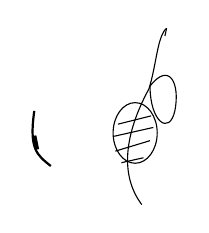
\begin{tikzpicture}[scale=.7]
\draw[line width=.8pt] (-1.6,1.0) .. controls (-1.7,.3) and (-1.55,.2) .. (-1.3,0);
\draw[line width=1.5pt] (-1.6,.55)--(-1.55,.3);
\draw (.35,-.7) .. controls (-.1,-.1) and (.1,.7) .. (.48,1.4) .. controls (.62,1.85) and (.63,2.35) .. (.8,2.5);
\draw (.8,2.5)--(.77,2.36);
\draw (.5,1.45) .. controls (.85,1.9) and (1.05,1.5) .. (.95,1.0) .. controls (.85,.55) and (.5,.8) .. (.5,1.45);
\draw (.23,.6) ellipse (.4 and .55);
\draw (-.08,.76)--(.52,.91) (-.15,.54)--(.56,.7) (-.13,.27)--(.5,.46) (-.02,.06)--(.38,.15);
\end{tikzpicture}}

\diagram{\begin{tikzcd}[ampersand replacement=\&]
-\widehat{\underline O}_x \& O_x\arrow[l]\arrow[d]\\
\unsure{\widehat{\widehat{\underline O}_{x|D}\otimes_{O_D}O_{D,x}|\widehat{\underline O}_D\otimes_{O_D}O_D}} \& O_D\arrow[l]\arrow[d]\\
\&\underline O_{\unsure{\eta|q}}
\end{tikzcd}}

\[
\operatorname{Hom}(K,\coprod_x\deleted{\unsure{I}} I_x)
\]

\diagram{\begin{tikzcd}[ampersand replacement=\&]
K\arrow[r] \& I_D\arrow[r] \& I_x\\
\widehat K_D^* \& \&\widehat O_{D,x}^*
\end{tikzcd}}
\figure{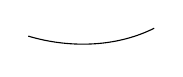
\begin{tikzpicture}\draw (0,.15).. controls (.5,0) and (1.1,0)..(1.6,.25);\end{tikzpicture}}

\diagram{\begin{tikzcd}[ampersand replacement=\&]
\widehat O_D\arrow[d] \& O_D\arrow[l]\arrow[d]\\
\widehat{\underline O}_{D,0} \& O_0\arrow[l]
\end{tikzcd}}

\diagram{\begin{tikzcd}[ampersand replacement=\&,column sep=large]
A_{[p_1>\cdots>p_n]}\&\\
A_{[p_n]}\arrow[u,"{\mathrm{hom\ local}}"]
\&\deleted{\unsure{A_{[p_n]}/p_{n+1}^k A_{[p_{\unsure{n}}]}}}\\
A_{p_n}\arrow[u,"{\mathrm{hom\ local}}"]\arrow[r]
\&A_{p_{n+1}}/p_{n+1}^k A_{p_{n+1}}
\end{tikzcd}}
% The abandoned arrow at the right of A_[p_n] is struck.
\[\deleted{\unsure{\longleftarrow|\longrightarrow}}\]
\diagram{\begin{tikzcd}[ampersand replacement=\&]
\deleted{A_{[p_1]}}\&\\
\deleted{A_{[p_2]}}\arrow[u]\arrow[r]\&\deleted{A_{[p_1]}}
\end{tikzcd}}

\diagram{\begin{tikzcd}[ampersand replacement=\&]
\displaystyle\prod_D\widehat O_D^{\unsure{*}}\&\displaystyle\sum\underline O_D\arrow[l]\\
\&K^{\unsure{*}}\\
\&O_D
\end{tikzcd}}

\[ A_{[p_1]}\qquad\underline A \]

\diagram{\begin{tikzcd}[ampersand replacement=\&]
\widehat{\underline O}_{D,x}\&\widehat{\underline O}_D\arrow[l]\arrow[d]\&\underline O_D\arrow[l,phantom,"{\unsure{\leftarrow|\twoheadleftarrow}}"]\arrow[d]\\
\deleted{\unsure{*}}\&\widehat K_D\&K^{\unsure{*}}\arrow[l]
\end{tikzcd}}

\diagram{\begin{tikzcd}[ampersand replacement=\&]
A_{p_1}\arrow[r]\& A_{\deleted{\unsure{p}}p_2}/p_2^k A_{p_2}
\end{tikzcd}}
